% Options for packages loaded elsewhere
\PassOptionsToPackage{unicode}{hyperref}
\PassOptionsToPackage{hyphens}{url}
%
\documentclass[
]{article}
\usepackage{lmodern}
\usepackage{amssymb,amsmath}
\usepackage{ifxetex,ifluatex}
\ifnum 0\ifxetex 1\fi\ifluatex 1\fi=0 % if pdftex
  \usepackage[T1]{fontenc}
  \usepackage[utf8]{inputenc}
  \usepackage{textcomp} % provide euro and other symbols
\else % if luatex or xetex
  \usepackage{unicode-math}
  \defaultfontfeatures{Scale=MatchLowercase}
  \defaultfontfeatures[\rmfamily]{Ligatures=TeX,Scale=1}
\fi
% Use upquote if available, for straight quotes in verbatim environments
\IfFileExists{upquote.sty}{\usepackage{upquote}}{}
\IfFileExists{microtype.sty}{% use microtype if available
  \usepackage[]{microtype}
  \UseMicrotypeSet[protrusion]{basicmath} % disable protrusion for tt fonts
}{}
\makeatletter
\@ifundefined{KOMAClassName}{% if non-KOMA class
  \IfFileExists{parskip.sty}{%
    \usepackage{parskip}
  }{% else
    \setlength{\parindent}{0pt}
    \setlength{\parskip}{6pt plus 2pt minus 1pt}}
}{% if KOMA class
  \KOMAoptions{parskip=half}}
\makeatother
\usepackage{xcolor}
\IfFileExists{xurl.sty}{\usepackage{xurl}}{} % add URL line breaks if available
\IfFileExists{bookmark.sty}{\usepackage{bookmark}}{\usepackage{hyperref}}
\hypersetup{
  pdftitle={lab10},
  pdfauthor={Ziyuan\_Han},
  hidelinks,
  pdfcreator={LaTeX via pandoc}}
\urlstyle{same} % disable monospaced font for URLs
\usepackage[margin=1in]{geometry}
\usepackage{color}
\usepackage{fancyvrb}
\newcommand{\VerbBar}{|}
\newcommand{\VERB}{\Verb[commandchars=\\\{\}]}
\DefineVerbatimEnvironment{Highlighting}{Verbatim}{commandchars=\\\{\}}
% Add ',fontsize=\small' for more characters per line
\usepackage{framed}
\definecolor{shadecolor}{RGB}{248,248,248}
\newenvironment{Shaded}{\begin{snugshade}}{\end{snugshade}}
\newcommand{\AlertTok}[1]{\textcolor[rgb]{0.94,0.16,0.16}{#1}}
\newcommand{\AnnotationTok}[1]{\textcolor[rgb]{0.56,0.35,0.01}{\textbf{\textit{#1}}}}
\newcommand{\AttributeTok}[1]{\textcolor[rgb]{0.77,0.63,0.00}{#1}}
\newcommand{\BaseNTok}[1]{\textcolor[rgb]{0.00,0.00,0.81}{#1}}
\newcommand{\BuiltInTok}[1]{#1}
\newcommand{\CharTok}[1]{\textcolor[rgb]{0.31,0.60,0.02}{#1}}
\newcommand{\CommentTok}[1]{\textcolor[rgb]{0.56,0.35,0.01}{\textit{#1}}}
\newcommand{\CommentVarTok}[1]{\textcolor[rgb]{0.56,0.35,0.01}{\textbf{\textit{#1}}}}
\newcommand{\ConstantTok}[1]{\textcolor[rgb]{0.00,0.00,0.00}{#1}}
\newcommand{\ControlFlowTok}[1]{\textcolor[rgb]{0.13,0.29,0.53}{\textbf{#1}}}
\newcommand{\DataTypeTok}[1]{\textcolor[rgb]{0.13,0.29,0.53}{#1}}
\newcommand{\DecValTok}[1]{\textcolor[rgb]{0.00,0.00,0.81}{#1}}
\newcommand{\DocumentationTok}[1]{\textcolor[rgb]{0.56,0.35,0.01}{\textbf{\textit{#1}}}}
\newcommand{\ErrorTok}[1]{\textcolor[rgb]{0.64,0.00,0.00}{\textbf{#1}}}
\newcommand{\ExtensionTok}[1]{#1}
\newcommand{\FloatTok}[1]{\textcolor[rgb]{0.00,0.00,0.81}{#1}}
\newcommand{\FunctionTok}[1]{\textcolor[rgb]{0.00,0.00,0.00}{#1}}
\newcommand{\ImportTok}[1]{#1}
\newcommand{\InformationTok}[1]{\textcolor[rgb]{0.56,0.35,0.01}{\textbf{\textit{#1}}}}
\newcommand{\KeywordTok}[1]{\textcolor[rgb]{0.13,0.29,0.53}{\textbf{#1}}}
\newcommand{\NormalTok}[1]{#1}
\newcommand{\OperatorTok}[1]{\textcolor[rgb]{0.81,0.36,0.00}{\textbf{#1}}}
\newcommand{\OtherTok}[1]{\textcolor[rgb]{0.56,0.35,0.01}{#1}}
\newcommand{\PreprocessorTok}[1]{\textcolor[rgb]{0.56,0.35,0.01}{\textit{#1}}}
\newcommand{\RegionMarkerTok}[1]{#1}
\newcommand{\SpecialCharTok}[1]{\textcolor[rgb]{0.00,0.00,0.00}{#1}}
\newcommand{\SpecialStringTok}[1]{\textcolor[rgb]{0.31,0.60,0.02}{#1}}
\newcommand{\StringTok}[1]{\textcolor[rgb]{0.31,0.60,0.02}{#1}}
\newcommand{\VariableTok}[1]{\textcolor[rgb]{0.00,0.00,0.00}{#1}}
\newcommand{\VerbatimStringTok}[1]{\textcolor[rgb]{0.31,0.60,0.02}{#1}}
\newcommand{\WarningTok}[1]{\textcolor[rgb]{0.56,0.35,0.01}{\textbf{\textit{#1}}}}
\usepackage{longtable,booktabs}
% Correct order of tables after \paragraph or \subparagraph
\usepackage{etoolbox}
\makeatletter
\patchcmd\longtable{\par}{\if@noskipsec\mbox{}\fi\par}{}{}
\makeatother
% Allow footnotes in longtable head/foot
\IfFileExists{footnotehyper.sty}{\usepackage{footnotehyper}}{\usepackage{footnote}}
\makesavenoteenv{longtable}
\usepackage{graphicx,grffile}
\makeatletter
\def\maxwidth{\ifdim\Gin@nat@width>\linewidth\linewidth\else\Gin@nat@width\fi}
\def\maxheight{\ifdim\Gin@nat@height>\textheight\textheight\else\Gin@nat@height\fi}
\makeatother
% Scale images if necessary, so that they will not overflow the page
% margins by default, and it is still possible to overwrite the defaults
% using explicit options in \includegraphics[width, height, ...]{}
\setkeys{Gin}{width=\maxwidth,height=\maxheight,keepaspectratio}
% Set default figure placement to htbp
\makeatletter
\def\fps@figure{htbp}
\makeatother
\setlength{\emergencystretch}{3em} % prevent overfull lines
\providecommand{\tightlist}{%
  \setlength{\itemsep}{0pt}\setlength{\parskip}{0pt}}
\setcounter{secnumdepth}{-\maxdimen} % remove section numbering

\title{lab10}
\author{Ziyuan\_Han}
\date{10/31/2021}

\begin{document}
\maketitle

\#Class 10: Halloween Mini-Project

\#\#Exploratory Analysis of Halloween Candy

\#1. Importing candy data
\#\url{https://raw.githubusercontent.com/fivethirtyeight/data/master/candy-powerranking/candy-data.csv}

\begin{Shaded}
\begin{Highlighting}[]
\NormalTok{candy_file <-}\StringTok{ "https://raw.githubusercontent.com/fivethirtyeight/data/master/candy-power-ranking/candy-data.csv"}
\NormalTok{candy =}\StringTok{ }\KeywordTok{read.csv}\NormalTok{(candy_file, }\DataTypeTok{row.names=}\DecValTok{1}\NormalTok{) }
\KeywordTok{head}\NormalTok{(candy)}
\end{Highlighting}
\end{Shaded}

\begin{verbatim}
##              chocolate fruity caramel peanutyalmondy nougat crispedricewafer
## 100 Grand            1      0       1              0      0                1
## 3 Musketeers         1      0       0              0      1                0
## One dime             0      0       0              0      0                0
## One quarter          0      0       0              0      0                0
## Air Heads            0      1       0              0      0                0
## Almond Joy           1      0       0              1      0                0
##              hard bar pluribus sugarpercent pricepercent winpercent
## 100 Grand       0   1        0        0.732        0.860   66.97173
## 3 Musketeers    0   1        0        0.604        0.511   67.60294
## One dime        0   0        0        0.011        0.116   32.26109
## One quarter     0   0        0        0.011        0.511   46.11650
## Air Heads       0   0        0        0.906        0.511   52.34146
## Almond Joy      0   1        0        0.465        0.767   50.34755
\end{verbatim}

\#Q1. How many different candy types are in this dataset?

85

\begin{Shaded}
\begin{Highlighting}[]
\KeywordTok{nrow}\NormalTok{(candy)}
\end{Highlighting}
\end{Shaded}

\begin{verbatim}
## [1] 85
\end{verbatim}

\#Q2. How many fruity candy types are in the dataset? The functions
dim(), nrow(), table() and sum() may be useful for answering the first 2
questions.

38

\begin{Shaded}
\begin{Highlighting}[]
\KeywordTok{nrow}\NormalTok{(candy[candy}\OperatorTok{$}\NormalTok{fruity }\OperatorTok{==}\StringTok{ }\DecValTok{1}\NormalTok{,])}
\end{Highlighting}
\end{Shaded}

\begin{verbatim}
## [1] 38
\end{verbatim}

\#What is your favorate candy?

\begin{Shaded}
\begin{Highlighting}[]
\NormalTok{candy[}\StringTok{"Twix"}\NormalTok{, ]}\OperatorTok{$}\NormalTok{winpercent}
\end{Highlighting}
\end{Shaded}

\begin{verbatim}
## [1] 81.64291
\end{verbatim}

\hypertarget{what-is-your-favorite-candy-in-the-dataset-and-what-is-its-winpercent-value}{%
\section{What is your favorite candy in the dataset and what is it's
winpercent
value?}\label{what-is-your-favorite-candy-in-the-dataset-and-what-is-its-winpercent-value}}

ReeseÕs Peanut Butter cup: winpercent is 84.18029

\begin{Shaded}
\begin{Highlighting}[]
\NormalTok{candy[}\StringTok{"ReeseÕs Peanut Butter cup"}\NormalTok{,]}\OperatorTok{$}\NormalTok{winpercent}
\end{Highlighting}
\end{Shaded}

\begin{verbatim}
## [1] 84.18029
\end{verbatim}

\#What is the winpercent value for ``Kit Kat''?

\begin{Shaded}
\begin{Highlighting}[]
\NormalTok{candy[}\StringTok{"Kit Kat"}\NormalTok{,]}\OperatorTok{$}\NormalTok{winpercent}
\end{Highlighting}
\end{Shaded}

\begin{verbatim}
## [1] 76.7686
\end{verbatim}

\#What is the winpercent value for ``Tootsie Roll Snack Bars

\begin{Shaded}
\begin{Highlighting}[]
\NormalTok{candy[}\StringTok{"Tootsie Roll Snack Bars"}\NormalTok{,]}\OperatorTok{$}\NormalTok{winpercent}
\end{Highlighting}
\end{Shaded}

\begin{verbatim}
## [1] 49.6535
\end{verbatim}

\begin{Shaded}
\begin{Highlighting}[]
\CommentTok{#install.packages("devtools") }
\CommentTok{#devtools::install_github("ropensci/skimr")}
\KeywordTok{library}\NormalTok{(}\StringTok{"skimr"}\NormalTok{)}
\KeywordTok{skim}\NormalTok{(candy)}
\end{Highlighting}
\end{Shaded}

\begin{longtable}[]{@{}ll@{}}
\caption{Data summary}\tabularnewline
\toprule
\endhead
Name & candy\tabularnewline
Number of rows & 85\tabularnewline
Number of columns & 12\tabularnewline
\_\_\_\_\_\_\_\_\_\_\_\_\_\_\_\_\_\_\_\_\_\_\_ &\tabularnewline
Column type frequency: &\tabularnewline
numeric & 12\tabularnewline
\_\_\_\_\_\_\_\_\_\_\_\_\_\_\_\_\_\_\_\_\_\_\_\_ &\tabularnewline
Group variables & None\tabularnewline
\bottomrule
\end{longtable}

\textbf{Variable type: numeric}

\begin{longtable}[]{@{}lrrrrrrrrrl@{}}
\toprule
skim\_variable & n\_missing & complete\_rate & mean & sd & p0 & p25 &
p50 & p75 & p100 & hist\tabularnewline
\midrule
\endhead
chocolate & 0 & 1 & 0.44 & 0.50 & 0.00 & 0.00 & 0.00 & 1.00 & 1.00 &
▇▁▁▁▆\tabularnewline
fruity & 0 & 1 & 0.45 & 0.50 & 0.00 & 0.00 & 0.00 & 1.00 & 1.00 &
▇▁▁▁▆\tabularnewline
caramel & 0 & 1 & 0.16 & 0.37 & 0.00 & 0.00 & 0.00 & 0.00 & 1.00 &
▇▁▁▁▂\tabularnewline
peanutyalmondy & 0 & 1 & 0.16 & 0.37 & 0.00 & 0.00 & 0.00 & 0.00 & 1.00
& ▇▁▁▁▂\tabularnewline
nougat & 0 & 1 & 0.08 & 0.28 & 0.00 & 0.00 & 0.00 & 0.00 & 1.00 &
▇▁▁▁▁\tabularnewline
crispedricewafer & 0 & 1 & 0.08 & 0.28 & 0.00 & 0.00 & 0.00 & 0.00 &
1.00 & ▇▁▁▁▁\tabularnewline
hard & 0 & 1 & 0.18 & 0.38 & 0.00 & 0.00 & 0.00 & 0.00 & 1.00 &
▇▁▁▁▂\tabularnewline
bar & 0 & 1 & 0.25 & 0.43 & 0.00 & 0.00 & 0.00 & 0.00 & 1.00 &
▇▁▁▁▂\tabularnewline
pluribus & 0 & 1 & 0.52 & 0.50 & 0.00 & 0.00 & 1.00 & 1.00 & 1.00 &
▇▁▁▁▇\tabularnewline
sugarpercent & 0 & 1 & 0.48 & 0.28 & 0.01 & 0.22 & 0.47 & 0.73 & 0.99 &
▇▇▇▇▆\tabularnewline
pricepercent & 0 & 1 & 0.47 & 0.29 & 0.01 & 0.26 & 0.47 & 0.65 & 0.98 &
▇▇▇▇▆\tabularnewline
winpercent & 0 & 1 & 50.32 & 14.71 & 22.45 & 39.14 & 47.83 & 59.86 &
84.18 & ▃▇▆▅▂\tabularnewline
\bottomrule
\end{longtable}

\#Q6. Is there any variable/column that looks to be on a different scale
to the majority of the other columns in the dataset? column 12 is
inscale. So we have to scale the data when doing PCA otherwise this
parameter is going to dominant over the rest.

\#Q7. What do you think a zero and one represent for the
candy\$chocolate column? 0 and 1 represent boolean values False and
True. Indicating the candy contains cholocate or not.

\#Q8. Plot a histogram of winpercent values

\begin{Shaded}
\begin{Highlighting}[]
\KeywordTok{library}\NormalTok{(ggplot2) }
\NormalTok{data =}\StringTok{ }\NormalTok{candy }
\NormalTok{data}\OperatorTok{$}\NormalTok{type =}\StringTok{ }\KeywordTok{rownames}\NormalTok{(data) }
\KeywordTok{ggplot}\NormalTok{(data, }\KeywordTok{aes}\NormalTok{(}\DataTypeTok{x=}\NormalTok{winpercent)) }\OperatorTok{+}\StringTok{ }\KeywordTok{geom_histogram}\NormalTok{()}
\end{Highlighting}
\end{Shaded}

\begin{verbatim}
## `stat_bin()` using `bins = 30`. Pick better value with `binwidth`.
\end{verbatim}

\includegraphics{lab10_files/figure-latex/unnamed-chunk-8-1.pdf} \#Q9.
Is the distribution of winpercent values symmetrical?

Yes

\#Q10. Is the center of the distribution above or below 50\%?

obove 50\%

\#Q11. On average is chocolate candy higher or lower ranked than fruit
candy? cholocate candy rank higher than fruit candy

\begin{Shaded}
\begin{Highlighting}[]
\KeywordTok{print}\NormalTok{(}\KeywordTok{mean}\NormalTok{(candy}\OperatorTok{$}\NormalTok{winpercent[}\KeywordTok{as.logical}\NormalTok{(candy}\OperatorTok{$}\NormalTok{chocolate)]))}
\end{Highlighting}
\end{Shaded}

\begin{verbatim}
## [1] 60.92153
\end{verbatim}

\begin{Shaded}
\begin{Highlighting}[]
\NormalTok{choc=data[data}\OperatorTok{$}\NormalTok{chocolate }\OperatorTok{==}\StringTok{ }\DecValTok{1}\NormalTok{,] }
\KeywordTok{ggplot}\NormalTok{(choc, }\KeywordTok{aes}\NormalTok{(}\DataTypeTok{x=}\NormalTok{winpercent)) }\OperatorTok{+}\StringTok{ }
\StringTok{  }\KeywordTok{geom_histogram}\NormalTok{() }\OperatorTok{+}\StringTok{ }\KeywordTok{xlim}\NormalTok{(}\DecValTok{0}\NormalTok{,}\DecValTok{100}\NormalTok{)}
\end{Highlighting}
\end{Shaded}

\begin{verbatim}
## `stat_bin()` using `bins = 30`. Pick better value with `binwidth`.
\end{verbatim}

\begin{verbatim}
## Warning: Removed 2 rows containing missing values (geom_bar).
\end{verbatim}

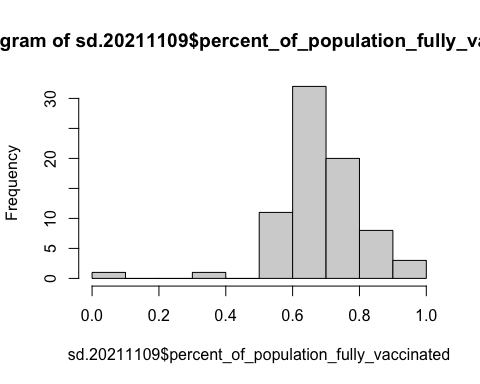
\includegraphics{lab10_files/figure-latex/unnamed-chunk-9-1.pdf}

\begin{Shaded}
\begin{Highlighting}[]
\NormalTok{fruit=data[data}\OperatorTok{$}\NormalTok{fruity }\OperatorTok{==}\StringTok{ }\DecValTok{1}\NormalTok{,] }
\KeywordTok{ggplot}\NormalTok{(fruit, }\KeywordTok{aes}\NormalTok{(}\DataTypeTok{x=}\NormalTok{winpercent)) }\OperatorTok{+}\StringTok{ }
\StringTok{  }\KeywordTok{geom_histogram}\NormalTok{() }\OperatorTok{+}\StringTok{ }\KeywordTok{xlim}\NormalTok{(}\DecValTok{0}\NormalTok{,}\DecValTok{100}\NormalTok{)}
\end{Highlighting}
\end{Shaded}

\begin{verbatim}
## `stat_bin()` using `bins = 30`. Pick better value with `binwidth`.
\end{verbatim}

\begin{verbatim}
## Warning: Removed 2 rows containing missing values (geom_bar).
\end{verbatim}

\includegraphics{lab10_files/figure-latex/unnamed-chunk-9-2.pdf} \#Q12.
Is this difference statistically significant? p-val of T-test is less
than 0.05, indicating there is statistical significance between
preferences for chocolate and fruity candy.

\begin{Shaded}
\begin{Highlighting}[]
\NormalTok{choc =}\StringTok{ }\NormalTok{candy}\OperatorTok{$}\NormalTok{winpercent[}\KeywordTok{as.logical}\NormalTok{(candy}\OperatorTok{$}\NormalTok{chocolate)] }
\NormalTok{fruit =}\StringTok{ }\NormalTok{candy}\OperatorTok{$}\NormalTok{winpercent[}\KeywordTok{as.logical}\NormalTok{(candy}\OperatorTok{$}\NormalTok{fruity)] }
\KeywordTok{t.test}\NormalTok{(choc, fruit)}
\end{Highlighting}
\end{Shaded}

\begin{verbatim}
## 
##  Welch Two Sample t-test
## 
## data:  choc and fruit
## t = 6.2582, df = 68.882, p-value = 2.871e-08
## alternative hypothesis: true difference in means is not equal to 0
## 95 percent confidence interval:
##  11.44563 22.15795
## sample estimates:
## mean of x mean of y 
##  60.92153  44.11974
\end{verbatim}

\#Overall Candy Rankings

\begin{Shaded}
\begin{Highlighting}[]
\KeywordTok{library}\NormalTok{(dplyr)}
\end{Highlighting}
\end{Shaded}

\begin{verbatim}
## 
## Attaching package: 'dplyr'
\end{verbatim}

\begin{verbatim}
## The following objects are masked from 'package:stats':
## 
##     filter, lag
\end{verbatim}

\begin{verbatim}
## The following objects are masked from 'package:base':
## 
##     intersect, setdiff, setequal, union
\end{verbatim}

\begin{Shaded}
\begin{Highlighting}[]
\NormalTok{candy }\OperatorTok\StringTok{ }\KeywordTok{arrange}\NormalTok{(winpercent) }\OperatorTok\StringTok{ }\KeywordTok{head}\NormalTok{(}\DecValTok{5}\NormalTok{)}
\end{Highlighting}
\end{Shaded}

\begin{verbatim}
##                    chocolate fruity caramel peanutyalmondy nougat
## Nik L Nip                  0      1       0              0      0
## Boston Baked Beans         0      0       0              1      0
## Chiclets                   0      1       0              0      0
## Super Bubble               0      1       0              0      0
## Jawbusters                 0      1       0              0      0
##                    crispedricewafer hard bar pluribus sugarpercent pricepercent
## Nik L Nip                         0    0   0        1        0.197        0.976
## Boston Baked Beans                0    0   0        1        0.313        0.511
## Chiclets                          0    0   0        1        0.046        0.325
## Super Bubble                      0    0   0        0        0.162        0.116
## Jawbusters                        0    1   0        1        0.093        0.511
##                    winpercent
## Nik L Nip            22.44534
## Boston Baked Beans   23.41782
## Chiclets             24.52499
## Super Bubble         27.30386
## Jawbusters           28.12744
\end{verbatim}

\begin{Shaded}
\begin{Highlighting}[]
\KeywordTok{head}\NormalTok{(candy[}\KeywordTok{order}\NormalTok{(candy}\OperatorTok{$}\NormalTok{winpercent),], }\DataTypeTok{n=}\DecValTok{5}\NormalTok{)}
\end{Highlighting}
\end{Shaded}

\begin{verbatim}
##                    chocolate fruity caramel peanutyalmondy nougat
## Nik L Nip                  0      1       0              0      0
## Boston Baked Beans         0      0       0              1      0
## Chiclets                   0      1       0              0      0
## Super Bubble               0      1       0              0      0
## Jawbusters                 0      1       0              0      0
##                    crispedricewafer hard bar pluribus sugarpercent pricepercent
## Nik L Nip                         0    0   0        1        0.197        0.976
## Boston Baked Beans                0    0   0        1        0.313        0.511
## Chiclets                          0    0   0        1        0.046        0.325
## Super Bubble                      0    0   0        0        0.162        0.116
## Jawbusters                        0    1   0        1        0.093        0.511
##                    winpercent
## Nik L Nip            22.44534
## Boston Baked Beans   23.41782
## Chiclets             24.52499
## Super Bubble         27.30386
## Jawbusters           28.12744
\end{verbatim}

\#Q13. What are the five least liked candy types in this set?

\begin{Shaded}
\begin{Highlighting}[]
\NormalTok{candy }\OperatorTok\StringTok{ }\KeywordTok{arrange}\NormalTok{(winpercent) }\OperatorTok\StringTok{ }\KeywordTok{head}\NormalTok{(}\DecValTok{5}\NormalTok{)}
\end{Highlighting}
\end{Shaded}

\begin{verbatim}
##                    chocolate fruity caramel peanutyalmondy nougat
## Nik L Nip                  0      1       0              0      0
## Boston Baked Beans         0      0       0              1      0
## Chiclets                   0      1       0              0      0
## Super Bubble               0      1       0              0      0
## Jawbusters                 0      1       0              0      0
##                    crispedricewafer hard bar pluribus sugarpercent pricepercent
## Nik L Nip                         0    0   0        1        0.197        0.976
## Boston Baked Beans                0    0   0        1        0.313        0.511
## Chiclets                          0    0   0        1        0.046        0.325
## Super Bubble                      0    0   0        0        0.162        0.116
## Jawbusters                        0    1   0        1        0.093        0.511
##                    winpercent
## Nik L Nip            22.44534
## Boston Baked Beans   23.41782
## Chiclets             24.52499
## Super Bubble         27.30386
## Jawbusters           28.12744
\end{verbatim}

\#Q14. What are the top 5 all time favorite candy types out of this set?

\begin{Shaded}
\begin{Highlighting}[]
\NormalTok{candy }\OperatorTok\StringTok{ }\KeywordTok{arrange}\NormalTok{(}\KeywordTok{desc}\NormalTok{(winpercent)) }\OperatorTok\StringTok{ }\KeywordTok{head}\NormalTok{(}\DecValTok{5}\NormalTok{)}
\end{Highlighting}
\end{Shaded}

\begin{verbatim}
##                           chocolate fruity caramel peanutyalmondy nougat
## ReeseÕs Peanut Butter cup         1      0       0              1      0
## ReeseÕs Miniatures                1      0       0              1      0
## Twix                              1      0       1              0      0
## Kit Kat                           1      0       0              0      0
## Snickers                          1      0       1              1      1
##                           crispedricewafer hard bar pluribus sugarpercent
## ReeseÕs Peanut Butter cup                0    0   0        0        0.720
## ReeseÕs Miniatures                       0    0   0        0        0.034
## Twix                                     1    0   1        0        0.546
## Kit Kat                                  1    0   1        0        0.313
## Snickers                                 0    0   1        0        0.546
##                           pricepercent winpercent
## ReeseÕs Peanut Butter cup        0.651   84.18029
## ReeseÕs Miniatures               0.279   81.86626
## Twix                             0.906   81.64291
## Kit Kat                          0.511   76.76860
## Snickers                         0.651   76.67378
\end{verbatim}

\#Q15. Make a first barplot of candy ranking based on winpercent values.
HINT: Use the aes(winpercent, rownames(candy)) for your first ggplot
like so:

\begin{Shaded}
\begin{Highlighting}[]
\KeywordTok{library}\NormalTok{(ggplot2) }
\KeywordTok{ggplot}\NormalTok{(candy) }\OperatorTok{+}
\KeywordTok{aes}\NormalTok{(}\DataTypeTok{x=}\NormalTok{winpercent, }\DataTypeTok{y=}\KeywordTok{rownames}\NormalTok{(candy)) }\OperatorTok{+}\StringTok{ }
\StringTok{  }\KeywordTok{geom_col}\NormalTok{()}
\end{Highlighting}
\end{Shaded}

\includegraphics{lab10_files/figure-latex/unnamed-chunk-14-1.pdf} \#Q16.
This is quite ugly, use the reorder() function to get the bars sorted by
winpercent? HINT: You can use aes(winpercent,
reorder(rownames(candy),winpercent)) to improve your plot.

\begin{Shaded}
\begin{Highlighting}[]
\KeywordTok{ggplot}\NormalTok{(candy) }\OperatorTok{+}
\KeywordTok{aes}\NormalTok{(winpercent, }\KeywordTok{reorder}\NormalTok{(}\KeywordTok{rownames}\NormalTok{(candy),winpercent)) }\OperatorTok{+}\StringTok{ }
\StringTok{  }\KeywordTok{geom_col}\NormalTok{()}
\end{Highlighting}
\end{Shaded}

\includegraphics{lab10_files/figure-latex/unnamed-chunk-15-1.pdf}

\begin{Shaded}
\begin{Highlighting}[]
\KeywordTok{ggplot}\NormalTok{(candy) }\OperatorTok{+}
\KeywordTok{aes}\NormalTok{(winpercent, }\KeywordTok{reorder}\NormalTok{(}\KeywordTok{rownames}\NormalTok{(candy),winpercent)) }\OperatorTok{+}\StringTok{ }
\StringTok{  }\KeywordTok{geom_col}\NormalTok{()}
\end{Highlighting}
\end{Shaded}

\includegraphics{lab10_files/figure-latex/unnamed-chunk-15-2.pdf} \#Q17.
What is the worst ranked chocolate candy? sixlets

\begin{Shaded}
\begin{Highlighting}[]
\KeywordTok{ggplot}\NormalTok{(candy) }\OperatorTok{+}
\KeywordTok{aes}\NormalTok{(winpercent, }\KeywordTok{reorder}\NormalTok{(}\KeywordTok{rownames}\NormalTok{(candy),winpercent)) }
\end{Highlighting}
\end{Shaded}

\includegraphics{lab10_files/figure-latex/unnamed-chunk-16-1.pdf}

\#Q18. What is the best ranked fruity candy? starburst

\#Taking a look at pricepercent

\begin{Shaded}
\begin{Highlighting}[]
\KeywordTok{library}\NormalTok{(ggrepel)}
\KeywordTok{aes}\NormalTok{(winpercent, pricepercent, }\DataTypeTok{label=}\KeywordTok{rownames}\NormalTok{(candy)) }\OperatorTok{+}\StringTok{ }
\StringTok{  }\KeywordTok{geom_text_repel}\NormalTok{(}\DataTypeTok{size=}\FloatTok{3.3}\NormalTok{, }\DataTypeTok{max.overlaps =} \DecValTok{5}\NormalTok{)}
\end{Highlighting}
\end{Shaded}

\begin{verbatim}
## NULL
\end{verbatim}

\#Q19. Which candy type is the highest ranked in terms of winpercent for
the least money - i.e.~offers the most bang for your buck? HersheyÕs
Krackel

\#Q20. What are the top 5 most expensive candy types in the dataset and
of these which is the least popular? Nik L Nip

\begin{Shaded}
\begin{Highlighting}[]
\NormalTok{ord <-}\StringTok{ }\KeywordTok{order}\NormalTok{(candy}\OperatorTok{$}\NormalTok{pricepercent, }\DataTypeTok{decreasing =} \OtherTok{TRUE}\NormalTok{) }
\KeywordTok{head}\NormalTok{( candy[ord,}\KeywordTok{c}\NormalTok{(}\DecValTok{11}\NormalTok{,}\DecValTok{12}\NormalTok{)], }\DataTypeTok{n=}\DecValTok{5}\NormalTok{ )}
\end{Highlighting}
\end{Shaded}

\begin{verbatim}
##                          pricepercent winpercent
## Nik L Nip                       0.976   22.44534
## Nestle Smarties                 0.976   37.88719
## Ring pop                        0.965   35.29076
## HersheyÕs Krackel               0.918   62.28448
## HersheyÕs Milk Chocolate        0.918   56.49050
\end{verbatim}

\#5 Exploring the correlation structure Now that we've explored the
dataset a little, we'll see how the variables interact with one another.
We'll use correlation and view the results with the corrplot package to
plot a correlation matrix.

\begin{Shaded}
\begin{Highlighting}[]
\KeywordTok{library}\NormalTok{(corrplot)}
\end{Highlighting}
\end{Shaded}

\begin{verbatim}
## corrplot 0.84 loaded
\end{verbatim}

\begin{Shaded}
\begin{Highlighting}[]
\NormalTok{cij <-}\StringTok{ }\KeywordTok{cor}\NormalTok{(candy) }
\KeywordTok{corrplot}\NormalTok{(cij)}
\end{Highlighting}
\end{Shaded}

\includegraphics{lab10_files/figure-latex/unnamed-chunk-19-1.pdf} \#Q22.
Examining this plot what two variables are anti-correlated (i.e.~have
minus values)? fruity and chocolate \#Q23. Similarly, what two variables
are most positively correlated? winpercent and chocolate

\#Principal Component Analysis

\begin{Shaded}
\begin{Highlighting}[]
\NormalTok{pca <-}\StringTok{ }\KeywordTok{prcomp}\NormalTok{(candy, }\DataTypeTok{scale.=}\OtherTok{TRUE}\NormalTok{) }
\KeywordTok{summary}\NormalTok{(pca)}
\end{Highlighting}
\end{Shaded}

\begin{verbatim}
## Importance of components:
##                           PC1    PC2    PC3     PC4    PC5     PC6     PC7
## Standard deviation     2.0788 1.1378 1.1092 1.07533 0.9518 0.81923 0.81530
## Proportion of Variance 0.3601 0.1079 0.1025 0.09636 0.0755 0.05593 0.05539
## Cumulative Proportion  0.3601 0.4680 0.5705 0.66688 0.7424 0.79830 0.85369
##                            PC8     PC9    PC10    PC11    PC12
## Standard deviation     0.74530 0.67824 0.62349 0.43974 0.39760
## Proportion of Variance 0.04629 0.03833 0.03239 0.01611 0.01317
## Cumulative Proportion  0.89998 0.93832 0.97071 0.98683 1.00000
\end{verbatim}

\begin{Shaded}
\begin{Highlighting}[]
\KeywordTok{plot}\NormalTok{(pca}\OperatorTok{$}\NormalTok{x[,}\DecValTok{1}\OperatorTok{:}\DecValTok{2}\NormalTok{])}
\end{Highlighting}
\end{Shaded}

\includegraphics{lab10_files/figure-latex/unnamed-chunk-20-1.pdf}

\begin{Shaded}
\begin{Highlighting}[]
\KeywordTok{plot}\NormalTok{(pca}\OperatorTok{$}\NormalTok{x[,}\DecValTok{1}\OperatorTok{:}\DecValTok{2}\NormalTok{], }\DataTypeTok{pch=}\DecValTok{16}\NormalTok{)}
\end{Highlighting}
\end{Shaded}

\includegraphics{lab10_files/figure-latex/unnamed-chunk-20-2.pdf}

\begin{Shaded}
\begin{Highlighting}[]
\NormalTok{my_data <-}\StringTok{ }\KeywordTok{cbind}\NormalTok{(candy, pca}\OperatorTok{$}\NormalTok{x[,}\DecValTok{1}\OperatorTok{:}\DecValTok{3}\NormalTok{])}
\NormalTok{p <-}\StringTok{ }\KeywordTok{ggplot}\NormalTok{(my_data) }\OperatorTok{+}
\KeywordTok{aes}\NormalTok{(}\DataTypeTok{x=}\NormalTok{PC1, }\DataTypeTok{y=}\NormalTok{PC2, }\DataTypeTok{size=}\NormalTok{winpercent}\OperatorTok{/}\DecValTok{100}\NormalTok{, }\DataTypeTok{text=}\KeywordTok{rownames}\NormalTok{(my_data), }\DataTypeTok{label=}\KeywordTok{rownames}\NormalTok{(my_data)) }
\NormalTok{p}
\end{Highlighting}
\end{Shaded}

\includegraphics{lab10_files/figure-latex/unnamed-chunk-20-3.pdf}

\begin{Shaded}
\begin{Highlighting}[]
\KeywordTok{library}\NormalTok{(ggrepel)}
\NormalTok{p }\OperatorTok{+}\StringTok{ }\KeywordTok{geom_text_repel}\NormalTok{(}\DataTypeTok{size=}\FloatTok{3.3}\NormalTok{, }\DataTypeTok{max.overlaps =} \DecValTok{7}\NormalTok{)}
\end{Highlighting}
\end{Shaded}

\begin{verbatim}
## Warning: ggrepel: 39 unlabeled data points (too many overlaps). Consider
## increasing max.overlaps
\end{verbatim}

\includegraphics{lab10_files/figure-latex/unnamed-chunk-20-4.pdf}

\begin{Shaded}
\begin{Highlighting}[]
\KeywordTok{theme}\NormalTok{(}\DataTypeTok{legend.position =} \StringTok{"none"}\NormalTok{) }\OperatorTok{+}\StringTok{ }\KeywordTok{labs}\NormalTok{(}\DataTypeTok{title=}\StringTok{"Halloween Candy PCA Space"}\NormalTok{,}\DataTypeTok{subtitle=}\StringTok{"Colored by type: chocolate bar (dark brown), chocolate other (light brown), fruity (red)"}\NormalTok{,}\DataTypeTok{caption=}\StringTok{"Data from 538"}\NormalTok{)}
\end{Highlighting}
\end{Shaded}

\begin{verbatim}
## List of 4
##  $ legend.position: chr "none"
##  $ title          : chr "Halloween Candy PCA Space"
##  $ subtitle       : chr "Colored by type: chocolate bar (dark brown), chocolate other (light brown), fruity (red)"
##  $ caption        : chr "Data from 538"
##  - attr(*, "class")= chr [1:2] "theme" "gg"
##  - attr(*, "complete")= logi FALSE
##  - attr(*, "validate")= logi TRUE
\end{verbatim}

\begin{Shaded}
\begin{Highlighting}[]
\KeywordTok{par}\NormalTok{(}\DataTypeTok{mar=}\KeywordTok{c}\NormalTok{(}\DecValTok{8}\NormalTok{,}\DecValTok{4}\NormalTok{,}\DecValTok{2}\NormalTok{,}\DecValTok{2}\NormalTok{)) }
\KeywordTok{barplot}\NormalTok{(pca}\OperatorTok{$}\NormalTok{rotation[,}\DecValTok{1}\NormalTok{], }\DataTypeTok{las=}\DecValTok{2}\NormalTok{, }\DataTypeTok{ylab=}\StringTok{"PC1 Contribution"}\NormalTok{)}
\end{Highlighting}
\end{Shaded}

\includegraphics{lab10_files/figure-latex/unnamed-chunk-20-5.pdf} \#Q24.
What original variables are picked up strongly by PC1 in the positive
direction? Do these make sense to you? HINT. pluribus means the candy
comes in a bag or box of multiple candies.

fruity, hard, pluribus. yes

\end{document}
